\documentclass{article}
\usepackage[utf8]{inputenc}
\usepackage{graphicx}
\usepackage{wrapfig}
\graphicspath{ {images/} }

\title{Math 150A Optimization Writing Project}
\author{David Feinzimer}
\date{June 25, 2017}

\begin{document}

\maketitle

\section{Description of Problem: The Least Expensive Path (Quickest Path)}

\begin{wrapfigure}{l}{0.25\textwidth}
    \centering
    
\includegraphics[width=0.25\textwidth]{title}
\end{wrapfigure}

Our problem is that with a limited amount of time we must run across campus to reach class.
Our destination is 1,000 feet south and 200 feet east of our current location.
When traveling southbound we can move at a rate of 10 feet per second.
When traveling eastbound we can move at a rate of 3 feet per second.
We have about four different paths to choose from but only one path with allow for the shortest trip to reach class.

Path 1 would first take us 1,000 feet southbound at 10 feet per second. However, we'd still need to travel 200 feet eastbound ultimately making this a costly option.

Path 2 would first take us 200 feet eastbound at 3 feet per second. However, we'd still need to travel 1,000 southbound through the quad at the equally slow speed of 3 feet per second making this path even more costly than path 1.

Path 3 would take us directly towards the classroom (as the bird flys) on a southeastern path at a slow rate of 3 feet per second but there would be no need to travel directly southbound followed by directly eastbound or vice versa.

A fourth (4) and final path would take us on a mixture of a pure southbound 10 foot per second stint followed by a slower 3 foot per second southeaster stint.

In the end, path 4 would be the best route to take. The rest of this paper will explain why that is and how I arrived at this conclusion.

\section{Theory And Process To Be Followed}

Modern day GPS systems and way-finding software specialize in solving this exact type of problem. The following is a description of the almost certain method these systems follow in order to deliver the most direct and efficient directions to their client's everyday.

While these advanced systems need to deal with real time data like constantly changing traffic patterns, our instance of this problem is a bit simpler as we have defined rates of speed that will not dynamically and constantly change on us.

Step 1) \t I will recognize, process, and give a label to all of the information that has been provided.

Step 2) \t I will recognized and explain the different relevant equations and their derivatives that will allow us to land at a correct answer. In this case I want to minimize time spent traveling to my class in McCarthy Hall.

Step 3) \t I will show all of the work involved in solving this specific way-finding problem.

\section{Processing \& Labeling Given Data}

In solving this problem it will help us to analyze and label our data as if we were looking at it on an X/Y coordinate plane.
From the problem, we are told we need to travel 1,000 feet south. Due to the face that the Y-axis traditionally runs north/south I will officially recognize our starting point as $ SRT $, an intersect on the Y-axis at (0,1000).
From the problem, we are also told we need to travel 200 feet east. Due to the face that the X-axis traditionally west/east I will recognize our ending point or destination as $ DST $, an intersect on the X-axis at (200,0). 
We are told a main walk-way runs north/south and allows travelers to move at a rate of 10 feet per second. Because the main walk-way runs north/south it lies along our Y-axis and because this is a rate of change on our Y-axis with respect to time we have $ \frac{dy}{dt} = 10\frac{ft}{sec} $ 
A quad also lies between us and class allowing travelers to only move at a rate of 3 feet per second. Because we will be traveling diagonally through the quad with reference to the Pythagorean Theorem which will be used later on this is a rate of change on our Z-axis with respect to time we have $ \frac{dz}{dt} = 3\frac{ft}{sec} $ 

\vspace{.5cm}
Given all of the above information we have the following variables:

\vspace{.25cm}
SRT @ (0,1000)

\vspace{.25cm}
DST @ (200,0)

\vspace{.25cm}
$ \frac{dy}{dt} = 10\frac{ft}{sec} $

\vspace{.25cm}
$ \frac{dz}{dt} = 3\frac{ft}{sec} $ 

\section{Recognizing Relevant Equations}

The first step is to build our basic function. With this problem, we are measuring an amount of time. Therefore we will define our function as $ TotalTime $. Our total time $ TotalTime $ to get to class is the time spent traveling southbound $ T(SB) $ plus the time spent traveling southeast $ T(SE) $. Therefore we will achieve our final answer with $ TotalTime = T(SB) + T(SE) $. It is also important to note that time itself is a ratio between distance and velocity, therefore $ T = \frac{distance}{velocity} $

\vspace{.5cm}
Given all of the above information we have the following equations:

\vspace{.25cm}
$ TotalTime = T(SB) + T(SE) $

\vspace{.25cm}
$ T = \frac{distance}{velocity} $

\vspace{.5cm}
Now we must further develop our $ TotalTime $ function into one that is solvable. With $ TotalTime = T(SB) + T(SE) $ we need to find the sum of $ T(SB) + T(SE) $

We know that in total, we need to travel 1000 feet south and 300 feet east to reach $ DST $.

If we let $ x $ represent the portion of our 1000 feet southern movement that will be spent traveling southeast, the portion of our trip spent traveling purely south can be represented by $ 1000 - x $. Since $ 100 - x $ represents the distance we will be traveling purely south we can place it over $ \frac{dy}{dt} $ to give us $ T(SB) $.

Now we must find $ T(SE) $. Since $ x $ represents the portion of our 1000 feet southern movement that will be spent traveling southeast and we need to travel 300 feet east we can use Pythagorean Theorem $ (a^2 + b^2 = c^2) $ to find $ T(SE) $. If we set $ a = x $ and $ b = 300 $ we have $ c = \sqrt{x^2 + 300^2} $. Since $ \sqrt{x^2 + 300^2} $ represents the distance we will be traveling southeast we can place it over $ \frac{dz}{dt} $ to give us $ T(SE) $.

\vspace{.5cm}
Following from the above information we have a complete equation for $ TotalTime $ and are ready to solve this equation.

\vspace{.25cm}
$ TotalTime = T(SB) + T(SE) = \frac{1000 - x}{10} + \frac{\sqrt{x^2 + 300^2}}{3} $

\section{Solving the Problem}

Step 1) Find the derivative of $ TotalTime $ or $ TotalTime' $:

\vspace{.5cm}
$ TotalTime = \frac{1000 - x}{10} + \frac{\sqrt{x^2 + 300^2}}{3} $

$= \frac{1000 - x}{10} + \frac{(x^2 + 300^2)^{1/2}}{3} $

\vspace{.5cm}
By the sum rule:

$TotalTime' = \frac{d}{dx} \big[ \frac{1000 - x}{10} \big] + \frac{d}{dx} \big[ \frac{(x^2 + 300^2)^{1/2}}{3} \big] $

$= -\frac{1}{10} + \frac{d}{dx} \big[ \frac{(x^2 + 300^2)^{1/2}}{3} \big] $

$= -\frac{1}{10} + \frac{(x^2 + 90,000)^{-1/2}x}{3} $

$= -\frac{1}{10} + \frac{\frac{1}{ (x^2 + 90,000)^{1/2} }x}{3} $

$= -\frac{1}{10} + \frac{x}{3(x^2 + 90,000)^{1/2}} $

$= \frac{x}{3(x^2 + 90,000)^{1/2}} -\frac{1}{10} $

\vspace{.5cm}
Step 2) Set  $ TotalTime' = 0 $ and solve for x:

$ 0 = \frac{x}{3(x^2 + 90,000)^{1/2}} -\frac{1}{10} $

$ \frac{1}{10} = \frac{x}{3(x^2 + 90,000)^{1/2}} $

$ 10x = 3\sqrt{x^2 + 90,000} $

$ (10x)^2 = (3\sqrt{x^2 + 90,000})^2 $

$ 100x^2 = (3^2) (x^2 + 90,000) $

$ 100x^2 = 9x^2 + 810,000 $

$ 0 = -91x^2 + 810,000 $

$ -91x^2 = -810,000 $

$ x^2 = \frac{810,000}{91} $

$ x = \sqrt{\frac{810,000}{91}} $

$ x = 94.34563530 $

\vspace{.5cm}
*Note* Because we're deciding how for we will travel purely south and because we're traveling a total southern distance of 1000 feet our $ x $ value needs to lie between 0 and 1000 feet or $ 0 \leq x \leq 1000 $

\vspace{.5cm}
Step 3) Test our three values of $ X $ ($ X = 0, 94.3456, 1000 $) on $ TotalTime $:

\vspace{.5cm}
$ TotalTime(0) = 200 seconds $

$ TotalTime(94.3456) = 195.39 seconds $

$ TotalTime(1000) = 348.01 seconds $

\vspace{.5cm}
Thus we can see we've found a minimum (time spent traveling to class) when $ x = 94.3456 $ and therefore the optimal route.

So, if this were a navigation system, it would recommend it's user to travel south along the main walk-way for $ (1000 - 94.3456) $ 905 feet before turning on a southeastern course for $ (\sqrt{94^2 + 300^2}) $ 314 feet to reach class in $ (\frac{195.39}{60}) $ 3 minutes and 15 seconds.

\centering
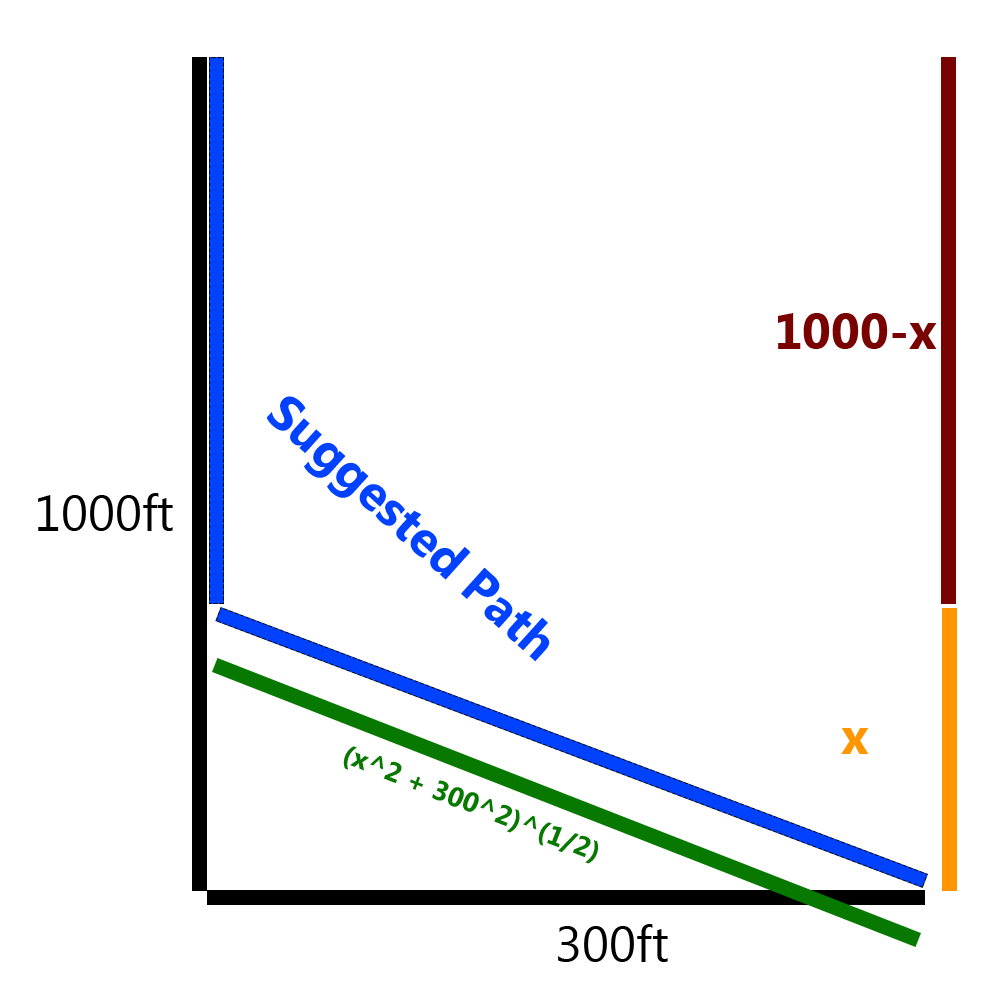
\includegraphics[width=6.5cm]{fig1}

\end{document}
